% !TeX root = ../../thesis.tex
\chapter{Introduction}\label{ch:introduction}

% Illustration on how to refer to your papers when using biblatex
% (see second line in thesis.tex to activate biblatex)
%\definecolor{shadecolor}{gray}{0.85}
%\begin{shaded}
%This chapter was previously published as:\\
%\fullcite{VandenBroeck2011IJCAI}
%\newpage
%\end{shaded}


The application of biodegradable metallic biomaterials \cite{Zheng2014, Liu2019, Han2019}, including magnesium \cite{Zhao2017,Zhen2013,Willumeit-Roemer2019}, zinc \cite{Venezuela2019,Mostaed2018}, and iron \cite{Schinhammer2010}, has become more prominent for over a decade in various biomedical engineering and tissue engineering disciplines. Among the mentioned materials, magnesium (Mg) is the most studied metals \cite{Esmaily2017}, the reason of which is its suitable mechanical and chemical properties for biomedical applications. Although poor corrosion resistance of Mg is a limiting factor for its application as a light structural material, like in transportation industry, it becomes an interesting characteristic when it comes to biodegradable materials field for cardiovascular and orthopedic applications \cite{Heublein2003,Staiger2006,Walker2014}. The first clinical usage of Mg was reported in 1878, but a renewed interest on it has grown significantly in the last 15-20 years \cite{Esmaily2017}. From the clinical and biomedical perspective, two major concerns about using Mg in clinics are the release of hydrogen gas and surface alkalization due to Mg dissolution \cite{Cecchinato2015}. These issues are commonly addressed addressed by alloying, biocompatible coating, and surface modification \cite{Esmaily2017}. 


\section{Chemistry of biodegradation of magnesium}


The biodegradation behavior of Mg is investigated in corrosion tests, in which the selection of the corrosive media plays an important role since it affects the underlying chemical reactions \cite{Mei2020}. By considering the main application of the biomaterial, which can be tissue engineering scaffolds, vascular stents, or orthopedic fixation implants, the corrosive media can be selected to be a representative of the service environment. The most basic form of the medium is a saline (NaCl) solution, in which the degradation rate is the highest possible \cite{Mei2020}. More complex solutions can be used to mimic the behavior of body environment by taking into account more body fluid components, the most popular of which are the Ringer's solution, PBS (phosphate buffered saline), SBFs (simulated body fluids), HBSS (Hank's balanced salt solution), and Earle's balanced salt solution (EBSS) \cite{Mei2020}. Adding more organic components to the solution will make it ready to simulate cell culture conditions. The common media for this purpose are MEM (Minimum Essential medium) and DMEM (Dulbecco's modified Eagle's medium) \cite{Mei2020}. Fig. \ref{fig:components} summarizes various commonly used electrolytes for testing biodegradable metals \cite{Mei2020}.


\begin{figure}
\centering
\medskip
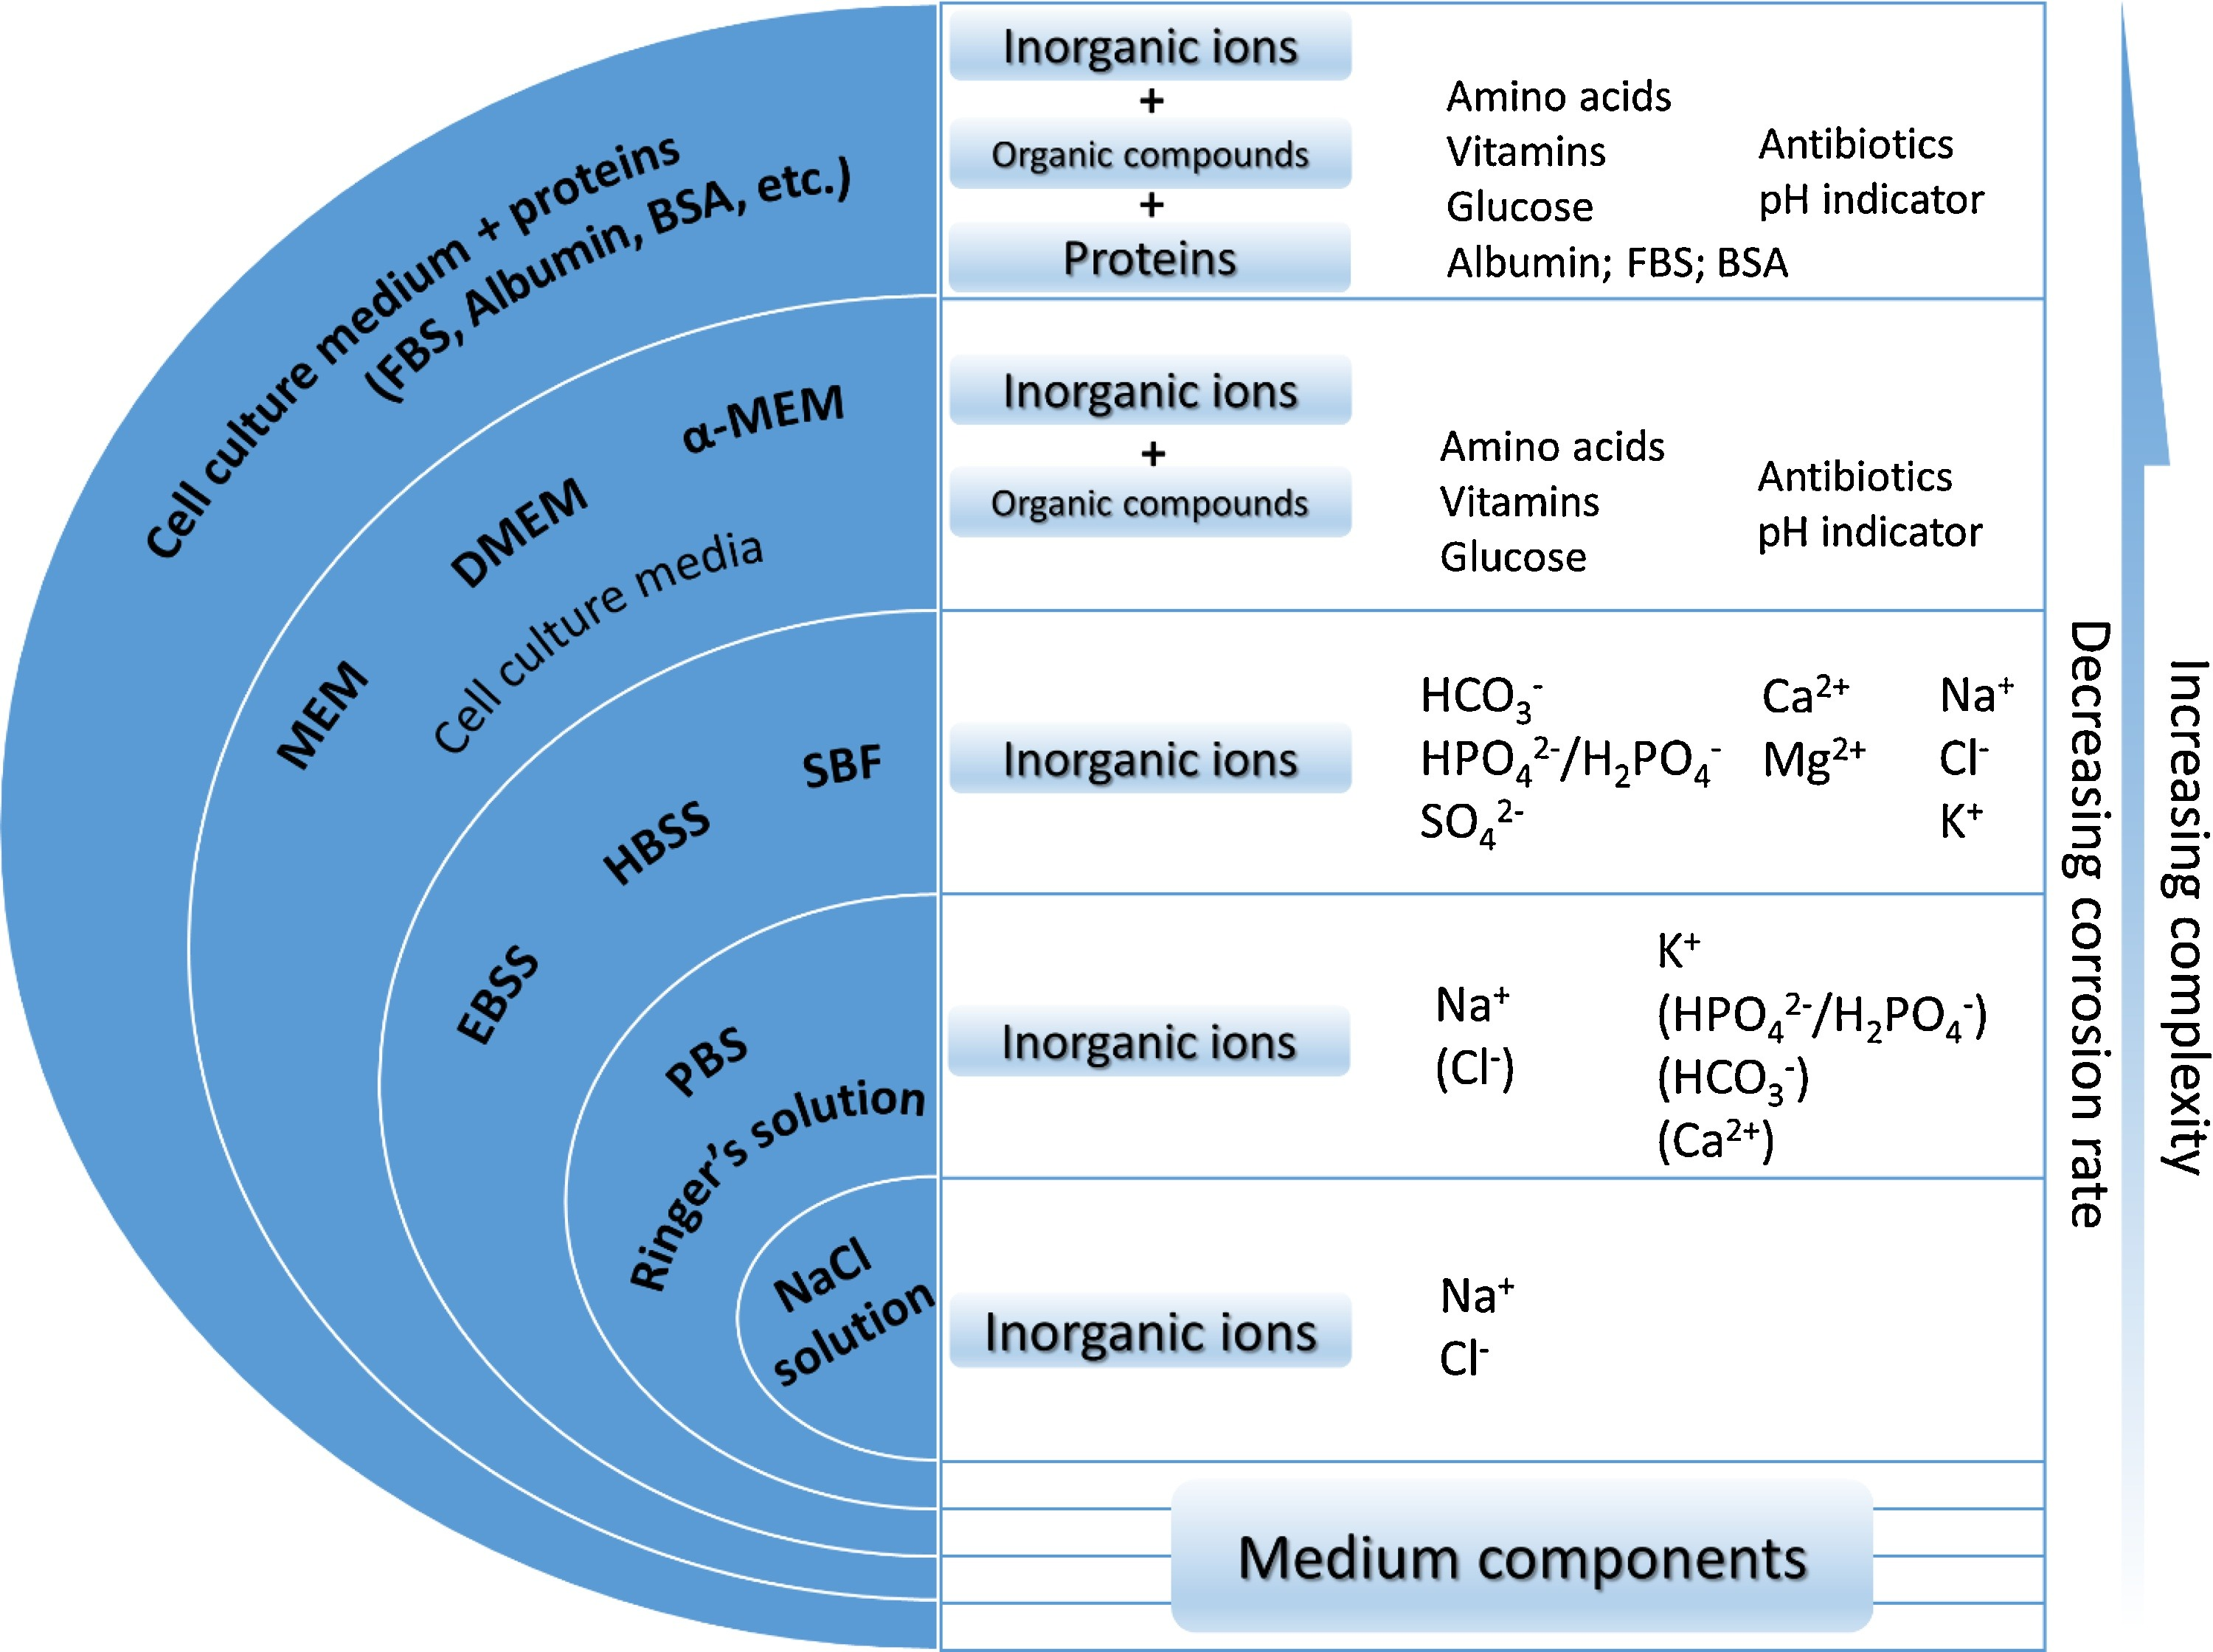
\includegraphics[width=1.0\textwidth]{components.jpg}
\caption[Commonly used electrolytes for testing biodegradable metals]{A schematic representation of commonly used electrolytes for testing biodegradable metals, sorted by their complexity from the chemical perspective from bottom to top \cite{Mei2020}.} 
\label{fig:components}
\end{figure}

A wide range of various studies have already investigated the effect of different components in the aforementioned corrosive media on the degradation behavior of Mg materials \cite{Mei2019,Zeng2014,Johnston2017, Lamaka2018,Mei2019a}. In addition to the presented chemical components, synthetic pH buffers (such as Tris as HEPES) has been shown to contribute to the biodegradation rate of Mg \cite{Mei2019}. The performed investigations on the effect of different inorganic components, including carbonate, phosphate, sulfate, and calcium, show the effective contribution of these components on the rate of degradation, although the corrosion protection resulted from the mutual effect of carbonate, phosphate and calcium has been more emphasized \cite{Mei2019,Lamaka2018}.




The most common solution for performing corrosion test on Mg is saline (NaCl) solution, in which the material undergoes an aggressive corrosion due to higher electrochemical activities \cite{Hadzima2014,Lu2019}. In a typical aqueous solution, the major corrosion reactions occurring can be written as \cite{Li2020,Atrens2015}:

Main, hydrogen evolution reaction (HER):
\begin{equation}
\mathrm{Mg}+2 \mathrm{H}_{2} \mathrm{O} \rightarrow \mathrm{Mg}(\mathrm{OH})_{2}+\mathrm{H}_{2} 
\end{equation}

Secondary, oxygen reduction reaction (ORR):
\begin{equation}
2 \mathrm{Mg}+2 \mathrm{H}_{2} \mathrm{O}+\mathrm{O}_{2} \rightarrow 2 \mathrm{Mg}(\mathrm{OH})_{2}
\end{equation}

In this situation, the corrosion products forming on the corroded surface of Mg consists mainly of $\mathrm{Mg}(\mathrm{OH})_{2}$ and $\mathrm{MgO}$, and the pH in regions close to this surface remains alkaline. In presence of chloride ions in the saline medium, the formed corrosion product may be broken or bypassed, leading to increased degradation rate:
\begin{equation} \label{eq:break_react_intro}
\mathrm{Mg}(\mathrm{OH})_{2}+2 \mathrm{Cl}^{-} \rightarrow \mathrm{Mg}^{2+}+2 \mathrm{Cl}^{-}+2 \mathrm{OH}^{-}
\end{equation}
\begin{equation} \label{eq:break_react_mgo_intro}
\mathrm{MgO}+ \mathrm{Cl}^{-} + \mathrm{H}_{2} \mathrm{O} \rightarrow \mathrm{Mg}^{2+}+ \mathrm{Cl}^{-}+ 2\mathrm{OH}^{-}
\end{equation}


The main advantage of using a saline solution for corrosion tests in comparison to more complex media is that absence of inorganic ions like carbonate, phosphate, sulfate, and calcium allows investigating the corrosion behavior without concerning possible contamination by microbial life. On the other hand, the main weakness of saline solution is that it cannot represent the complexity of real body fluid, and as a result, a more complex medium is required to investigate such conditions. To address this issue, more complex saline solutions, such as PBS are widely used for assessing the applicability of Mg alloys in more complex conditions from the chemical perspective \cite{Schille2011,Xue2012}. Despite the mentioned limitations, corrosion test in saline solution is beneficial for understanding intrinsic degradation properties of Mg. 


The term "simulated body fluid" is generally used to refer to solutions containing inorganic ions of human serum and interstitial fluid in corrosion tests \cite{Mei2020}. The commonly used media in this regard are SBF, HBSS, and EBSS, which include the same inorganic components with a slight difference in their concentrations. A typical composition of these media is chloride, carbonate, phosphates, sulfate, and calcium. The individual effect of these components on the rate of degradation of Mg has been extensively studied, in which it has been observed that carbonate and phosphate slow down the rate while the effect of sulfate is negligible \cite{Johnston2017,Mei2019a}. The concentration of $\mathrm{HCO}_{3}^{-}$ affects the pH buffering capacity and the degradation rate of Mg simultaneously \cite{Xin2011}. The effect of calcium ion is more complex because it doesn't contribute to the Mg corrosion directly. Fig. \ref{fig:reactions_intro} briefly summarizes the various reactions and formed precipitation compositions of the mentioned media for testing the degradation behavior of Mg \cite{Mei2020}.


\begin{figure}
\centering
\medskip
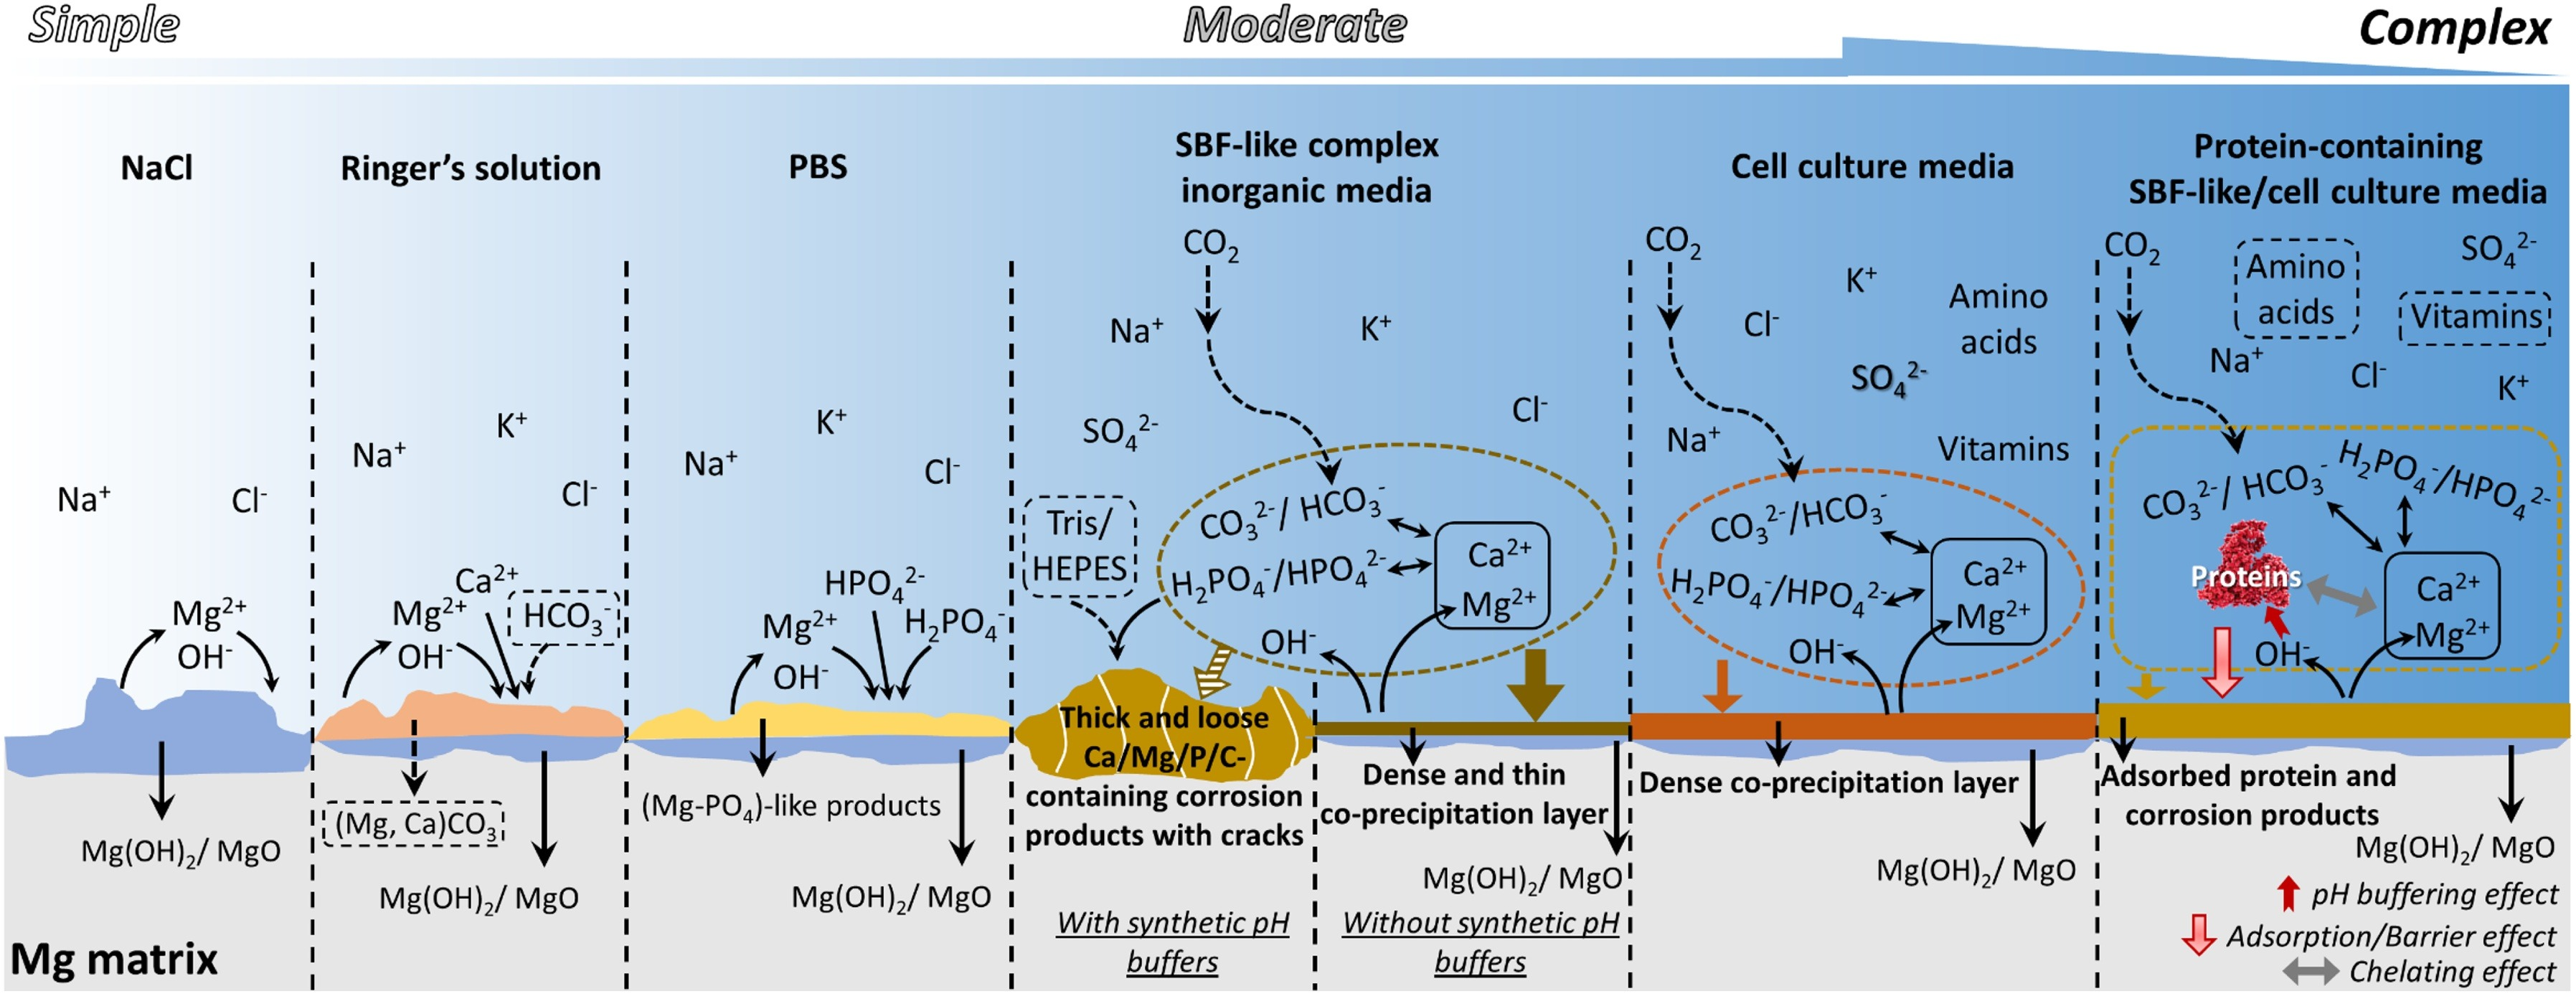
\includegraphics[width=1.0\textwidth]{reactions.jpg}
\caption[Mg biodegradation behavior in commonly used test solutions]{A schematic representation of Mg biodegradation behavior in commonly used solutions for corrosion tests of biodegradable metals \cite{Mei2020}.} \label{fig:reactions_intro}
\end{figure}



\subsection{Degradation rate evaluation techniques}

Generally speaking, the method used for evaluating the degradation rate can affect the reported behavior. For example, it has been shown that in HBSS, the measured corrosion rate of Mg is lower (slower) when evaluated using  hydrogen evolution in comparison to the rate found by direct weight loss measurements \cite{Johnston2015,Johnston2019}, which can be due to the secondary dissolution of evolved hydrogen. Moreover, the consumption of oxygen due to secondary ORR can affect the volume of evolved gas, which is more significant for media with slower degradation rate such as HBSS and MEM \cite{Wang2020}. Table \ref{tab:methods_intro} summarizes the advantages and shortcomings of widely used techniques for measuring degradation rate \cite{Mei2020}. 


\begin{table}[h]
\caption{Summary of various common methods to asses the degradation rate of Mg}
\medskip
\resizebox{\textwidth}{!}{%
\begin{tabular}{p{0.3\textwidth}p{0.5\textwidth}p{0.5\textwidth}}
\hline
Test method &
  Advantages &
  Shortcomings \\ \hline
Weight loss &
  \begin{tabular}[p{0.4\textwidth}]{@{}p{0.45\textwidth}}High reliability\\ Direct measurement\\ Easily controlled test environment\end{tabular} &
  \begin{tabular}[p{0.4\textwidth}]{@{}p{0.45\textwidth}}Non-continuous. Does not reveal varying corrosion rate throughout the immersion\\ Low sensitivity at the initial stages\end{tabular} \\ \hline
Hydrogen evolution &
  \begin{tabular}[p{0.4\textwidth}]{@{}p{0.45\textwidth}}Continuous\\ Can be automated\\ Can be performed in closed eudiometers\end{tabular} &
  \begin{tabular}[p{0.4\textwidth}]{@{}p{0.45\textwidth}}Performed in open environment in most cases\\ Might show underestimated values of corrosion rate due to secondary ORR and solubility of H2 in aqueous media\end{tabular} \\ \hline
Potentiodynamic polarization &
  Fast measurement &
  \begin{tabular}[p{0.4\textwidth}]{@{}p{0.45\textwidth}}Non-continuous\\ Open environment measurement in most cases\\ Very often low correlation with long-term weight loss measurements\end{tabular} \\ \hline
Electrochemical impedance spectroscopy &
  \begin{tabular}[p{0.4\textwidth}]{@{}p{0.45\textwidth}}Continuous\\ In situ investigation of protective properties of forming corrosion products\end{tabular} &
  Performed in open environment in most cases
\\  \hline
\end{tabular}}
\label{tab:methods_intro}
\end{table}





% Some dummy code to get at least 1 entry in the nomenclature.
\nomenclature{$\Theta$}{A nice symbol}
Introducing some symbol: $\Theta$.

% Some dummy code to get at least 1 entry in the list of
% abbreviations.
\newglossaryentry{md}{name={MD},description={molecular dynamics}}
Introducing an acronym: \gls{md}.




%%%%%%%%%%%%%%%%%%%%%%%%%%%%%%%%%%%%%%%%%%%%%%%%%%
% Keep the following \cleardoublepage at the end of this file, 
% otherwise \includeonly includes empty pages.
\cleardoublepage

% vim: tw=70 nocindent expandtab foldmethod=marker foldmarker={{{}{,}{}}}
